\section{Experiments}
\label{sec:evidence}

The two accounts agree that gaps shrink with $\sigma$ and order
by severity; everything else is discriminating, and each subsection
below states the prediction it discharges, against criteria frozen
before the runs, together with its designated probe, several of
which double as falsifiers of the account's own assumptions. The
experiments proceed one term at a time: the instrument, its validation,
and the debiased verdict map it certifies (\S\ref{sec:instrument}); the
spectral family scored against that map at the boundary level
(\S\ref{sec:phenomenon}); the graph floor (\S\ref{sec:floor}); the data
branch and its governors (\S\ref{sec:anatomy}); the floor's
decomposition (\S\ref{sec:decomposition}); and the account confronted
with held-out routes (\S\ref{sec:confronted}, Fig.~\ref{fig:e5}).

\subsection{The instrument and the debiased verdict map}
\label{sec:instrument}

\begin{figure}[t]
\centering
\begin{subfigure}[t]{0.46\textwidth}
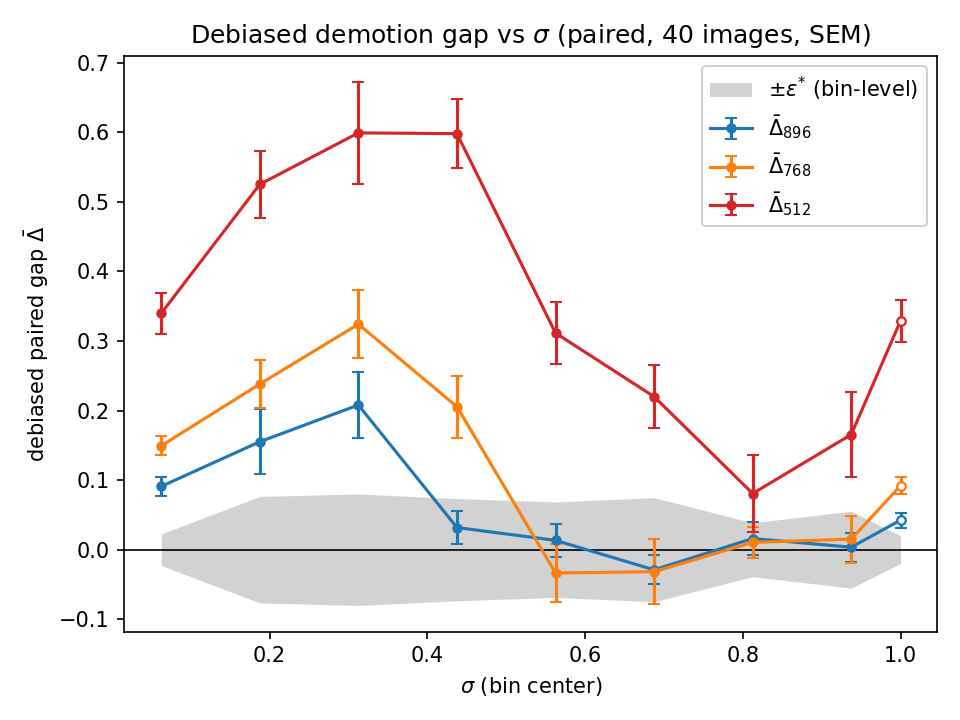
\includegraphics[width=\linewidth]{figs/gap_debiased.png}
\phantomcaption
\label{fig:gapcurves}
\end{subfigure}\hfill
\begin{subfigure}[t]{0.515\textwidth}
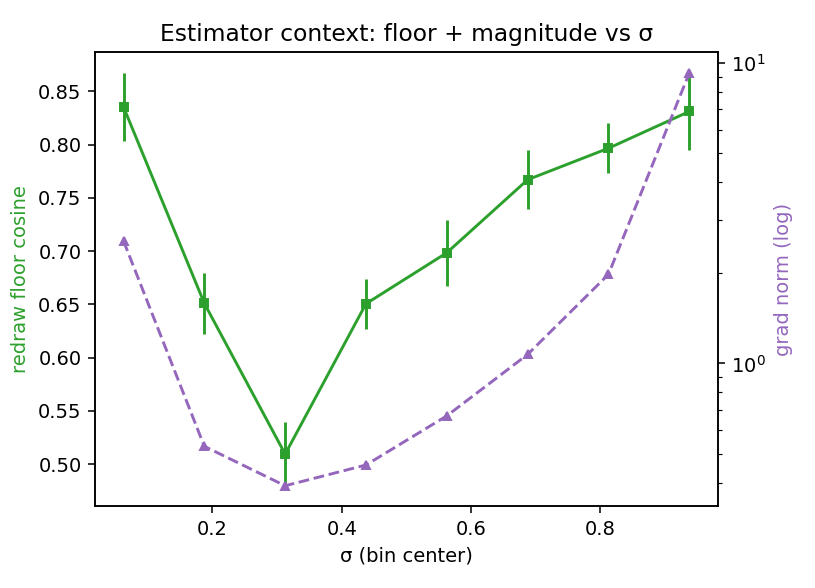
\includegraphics[width=\linewidth]{figs/estimator_context.png}
\phantomcaption
\label{fig:estimator}
\end{subfigure}
\caption{The verdict, before the apparatus.
(a)~Debiased demotion gap per $\sigma$-bin, paired against the
re-encoding control ($1024$-tier natives, $N{=}40$; values in
Table~\ref{tab:debiasedmap}; gray band: bin-level $\pm\epsstar$,
Eq.~\ref{eq:safe}; open markers: the $\sigma{=}1$ endpoint bin):
safety is a per-route boundary (the $896$ route enters the band at
$\sigma \approx 0.5$, $768$ has no certifiable window, and $512$ does
not enter at any noise level), against the spectral family's prediction
of $\sigma \approx 0.14$--$0.20$ (Fig.~\ref{fig:spectrum},
\S\ref{sec:phenomenon}).
(b)~The estimator context those curves are read through: the
redraw-floor cosine and the U-shaped gradient norm
$\|\bar g_{\src}(\sigma)\|$ (\S\ref{sec:anatomy}).}
\label{fig:verdict}
\end{figure}

\begin{figure}[t]
\centering
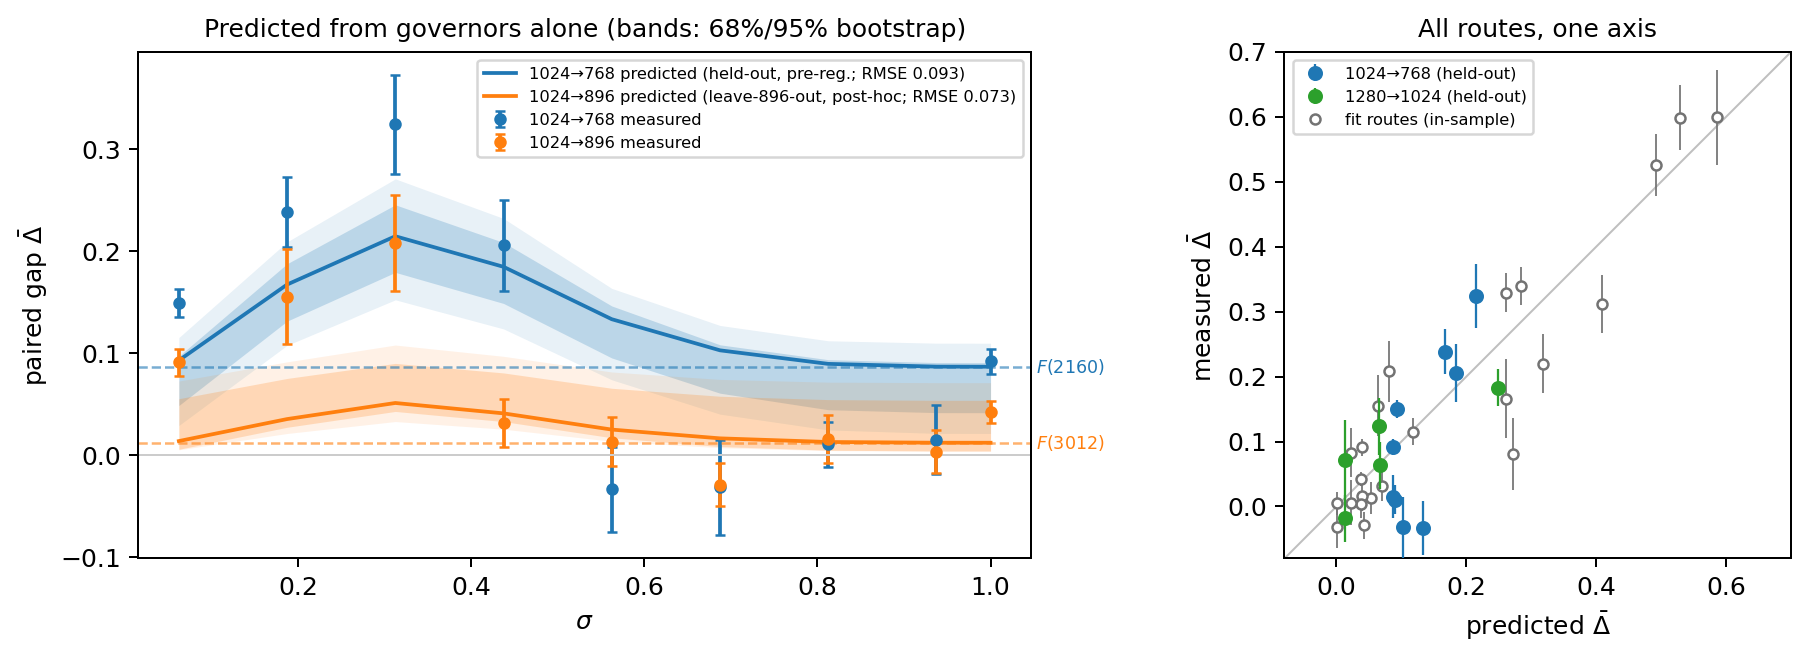
\includegraphics[width=\linewidth]{figs/e5_main.png}
\caption{The account as a predictive theory (discharged in
\S\ref{sec:confronted}), under the headline exact angular link
(Eq.~\ref{eq:exact}; the three-form comparison is Appendix
Fig.~\ref{fig:e51280}). Left: $1024$-tier predictions with zero
per-route freedom: the pre-registered held-out route $1024{\to}768$,
and $1024{\to}896$ under the post-hoc leave-$896$-out re-derivation (so
labeled; governors from $512{+}1120$ alone). Dashed: each route's
predicted floor $F(n)$; the gap between dashed and solid is the data
term. Bands: $68\%/95\%$ full-pipeline bootstrap (resample images
$\to$ re-bin $\to$ refit $\to$ re-derive governors $\to$ re-predict;
$B{=}1000$; $\bar m$ and $\|\bar g_{\src}\|$ are run-level instruments, held fixed).
The $768$ mid-$\sigma$ dip sits outside the $95\%$ band
(\S\ref{sec:confronted}). Right: predicted vs measured across all five
routes and bins under the pre-registered pipeline; filled: the two
held-out routes; open: fit routes (in-sample).}
\label{fig:e5}
\end{figure}

\paragraph{What we will show.}
Figure~\ref{fig:verdict} is the paper's central measurement, stated
before the apparatus that produced it. Panel~(a) is the debiased
demotion gap per $\sigma$-bin (the per-route excess over the
re-encoding control, in cosine units) for $1024$-tier natives
demoted to $896/768/512$: the mildest route becomes safe only from
$\sigma \approx 0.5$, the $768$ route is not certified at any noise
level, and the
$2\times$ downscale is gapped at every noise level, including
pure-noise input. Panel~(b) is the context every such number is read
through: the redraw-floor cosine, which is what finite draws do to the
estimator, and the U-shaped gradient norm $\|\bar g_{\src}(\sigma)\|$ that shapes
the curves (\S\ref{sec:anatomy}). The rest of this subsection builds
the instrument behind the figure: the model and probe, the verdict
table the figure plots, and the finite-draw ablation that forces every
number in this paper into debiased units.

\paragraph{Model and data.}
All measurements use Anima \citep{circlestone2025anima}, an open
DiT-based flow-matching text-to-image model (2B parameters, 28
transformer blocks, 3D rotary position embeddings, and the Qwen-Image
VAE, \citealp{wu2025qwenimage}), fine-tuned with LoRA adapters on an
illustration corpus. Images are
bucketed by native aspect ratio into resolution \emph{tiers} indexed by
nominal edge length $e \in \{512, 768, 896, 1024, 1280\}$; a tier-$e$ image
occupies roughly $(e/16)^2$ latent-patch tokens (e.g.\ ${\sim}4{,}100$
tokens at 1024, ${\sim}3{,}000$ at 896, ${\sim}2{,}160$ at 768,
${\sim}1{,}000$ at 512). The probe adapter is a plain LoRA checkpoint
trained at native tiers; we return to this operating-point dependence in
\S\ref{sec:limitations}.

\paragraph{The gradient probe.}
For each image and each of $B$ uniform $\sigma$-bins we accumulate adapter
gradients over $D$ stratified noise draws per arm (verdict runs:
$8 \times 8$ unless noted; $N = 40$ images) and compare arms by cosine
similarity of the flattened accumulated gradients:
\begin{itemize}
\item \textbf{floor}: two independent draw sets at native resolution,
the redraw null;
\item \textbf{reenc}: decode--re-encode at native resolution, the
control of \S\ref{sec:estimand};
\item \textbf{demote arms}: one per edge $e$ under test;
\item \textbf{self-floors} (debiased runs): the per-arm second
independent draw set the debiased estimator of \S\ref{sec:debias}
requires.
\end{itemize}
The gap is in cosine units (a mismatch \emph{fraction}, scale-free;
bin-mean SEM ${\sim}0.02$ at $N{=}40$). Gap subtraction, not absolute
cosines, is the valid read: the floor itself moves with $\|g\|$ across
bins. Every bin-mean curve must pass a split-half reliability check over
images, a discipline imposed after an earlier failure in which
per-image rankings from the same gradients had split-half reliability
indistinguishable from zero. Uniform $\sigma$-bins make the
training-time $\sigma$-density irrelevant to the map; density-weighting
the bins reproduces our earlier pooled measurements as a consistency
check. Estimator details and the endpoint / x-zero probe modes are in
Appendix~\ref{app:instrument}.

\paragraph{The measurement.}
Table~\ref{tab:debiasedmap} gives the debiased verdict map for
$1024$-tier natives demoted to $896/768/512$, the numbers plotted in
Fig.~\ref{fig:gapcurves} (the uncorrected historical
curves are Appendix Table~\ref{tab:phase0}).

\begin{table}[t]
\caption{\textbf{Debiased verdict map} (plotted in
Fig.~\ref{fig:gapcurves}): paired per-image debiased excess
$\bgap$ (SEM) against the re-encoding control, $1024$-tier natives
($N{=}40$, $D{=}8$/bin plus a $\sigma{=}1$ endpoint bin at the same
draws; non-finite and $|\gap_{e,i}| > 1.5$ per-image values trimmed,
retaining $35$--$40$ images per cell). Bin-level $\epsstar$ at this
$(N, D)$ is $0.03$--$0.08$ (Eq.~\ref{eq:safe}).}
\label{tab:debiasedmap}
\centering
\small
\begin{tabular}{cccc}
\toprule
$\sigma$ bin center & $1024{\to}896$ & $1024{\to}768$ & $1024{\to}512$ \\
\midrule
0.06 & $+.091$ {\scriptsize(.013)} & $+.149$ {\scriptsize(.014)} & $+.340$ {\scriptsize(.029)} \\
0.19 & $+.155$ {\scriptsize(.047)} & $+.238$ {\scriptsize(.034)} & $+.525$ {\scriptsize(.048)} \\
0.31 & $+.208$ {\scriptsize(.047)} & $+.324$ {\scriptsize(.049)} & $+.599$ {\scriptsize(.073)} \\
0.44 & $+.032$ {\scriptsize(.024)} & $+.206$ {\scriptsize(.045)} & $+.598$ {\scriptsize(.050)} \\
0.56 & $+.013$ {\scriptsize(.024)} & $-.034$ {\scriptsize(.042)} & $+.312$ {\scriptsize(.045)} \\
0.69 & $-.029$ {\scriptsize(.021)} & $-.032$ {\scriptsize(.047)} & $+.220$ {\scriptsize(.046)} \\
0.81 & $+.016$ {\scriptsize(.024)} & $+.011$ {\scriptsize(.022)} & $+.081$ {\scriptsize(.056)} \\
0.94 & $+.004$ {\scriptsize(.021)} & $+.015$ {\scriptsize(.034)} & $+.166$ {\scriptsize(.061)} \\
\midrule
1.0 (endpoint) & $+.043$ {\scriptsize(.011)} & $+.092$ {\scriptsize(.012)} & $+.329$ {\scriptsize(.030)} \\
\bottomrule
\end{tabular}
\end{table}

Three reads, against criteria frozen before the runs:
(i)~$\sigma$-dependence is real and in the predicted direction, and tier
ordering holds at every bin: the \emph{qualitative} spectral
intuition survives;
(ii)~the crossover for the mildest route is $\sigma \approx 0.5$
(the $896$ route is clearly gapped through $\sigma \le 0.31$, marginal
at $0.44$, and its means sit within $\pm 0.03$ of zero from $0.56$ on),
$3.5\times$ the equal-power prediction; no tolerance rescues the
spectral family, a boundary-level score deferred to
\S\ref{sec:phenomenon} (Table~\ref{tab:null});
(iii)~the $2\times$ downscale route is \emph{certifiably unsafe at every
noise level}: its paired debiased lower bound stays above $\epsstar$ in
every bin (means $+0.08$ to $+0.60$), including $+0.17 \pm 0.06$ at
$\sigma = 0.94$, where the input is ${\sim}97\%$ noise by power in every
band the coarse grid cannot represent, a high-$\sigma$ persistence
that no member of the spectral family can produce. There is no noise level at which a
$2\times$-downscaled latent yields the native gradient.

Two revisions against the historical record are part of the result. The
$768$ route's high-$\sigma$ plateau was roughly half estimator bias:
debiased means sit within noise of zero across $\sigma \in [0.56,
0.94]$, but with upper bounds that do not cross below the $0.02$ margin
at this $(N, D)$, and a real endpoint floor of $+0.092 \pm 0.012$
remains; the earlier verdict of ``unsafe at every noise level''
accordingly softens to \emph{no certifiable window at
instrument resolution} (\S\ref{sec:map}). Conversely the $896$ route's
endpoint shows a small \emph{real} gap ($+0.042 \pm 0.011$) that
single-estimate variance had buried; its safe window is the interior
$\sigma \in (0.5, 0.94]$, not the endpoint itself.

\paragraph{Does finite-draw bias matter?}
The bias mechanism of \S\ref{sec:debias} is live at our operating
point, and large. A variance back-of-envelope predicts spurious
endpoint gaps of ${\approx}\,0.02 / 0.05 / 0.15$ for $896/768/512$
(plausibly ${\sim}40\%$ of the uncorrected intermediate floors), and a
retroactive scan confirms the confound: the $1024{\to}896$ endpoint gap
decays as ${+}0.100 / {+}0.035 / {-}0.016$ at $D = 4/8/16$, a clean
$c/D$ decay with fitted $c \approx 0.5$. The native floor itself makes
the point sharpest: at $D{=}8$--$16$ the uncorrected endpoint
self-cosine reads $0.79$--$0.85$, but a nested draw sweep
($D = 4 \ldots 64$) extrapolates it to $1.005$ (bootstrap 95\% CI
$[0.994, 1.016]$): the population-level per-bin native gradient is a
\emph{fixed direction}, and the entire redraw floor is finite-draw
noise, not intrinsic gradient stochasticity. No conclusion in this
paper survives on the naive estimator alone.

\paragraph{The debiased estimator, operated.}
Endpoint-mode runs sweep nested draw prefixes
$D \in \{4, 8, 16, 32, 64\}$ (the $D{=}64$ pass contains the smaller
draw sets, so one set of forwards suffices) and fit
$\gap(D) = \gap_\infty + c/D$ per route with a bootstrap CI over
images; verdict-grid runs compute Eq.~\ref{eq:debias} per image and
bin. The mutual check of \S\ref{sec:debias} passes: debiased fits are
$D$-flat ($|c| \le 0.05$ for the $512$ route, against
$c \approx +0.29$ uncorrected), so the attenuation correction removes
exactly the $1/D$ component the sweep isolates.
One caveat delimits where Eq.~\ref{eq:debias} is readable. At $D{=}8$
per bin, the \emph{unpaired} debiased estimator is unstable in bins
where the floors themselves are small (mid-$\sigma$; the denominator is
noisy): there the readable object is the \emph{paired per-image excess}
$\gap_{e,i} = \dgap_{e,i} - \dgap_{\reenc,i}$ of \S\ref{sec:estimand},
with non-finite and $|\gap_{e,i}| > 1.5$ values trimmed; pairing cancels
the shared per-image, per-bin draw structure. All verdict maps below
report this paired object. Finite-draw cosines are also
compiler-kernel-path sensitive, so all pairings live within one run
(Appendix~\ref{app:instrument}).

\paragraph{Measured resolution.}
At the verdict grid's operating point ($N{=}40$, $D{=}8$/bin) the
bin-level $\epsstar$ (Eq.~\ref{eq:safe}) is $0.03$--$0.08$;
endpoint-mode draw sweeps ($D$ up to $64$) tighten it to
${\approx}\,0.01$--$0.02$.

\paragraph{Units and coverage, stated once.}
Every number in the main text is debiased; the
uncorrected historical tables are in Appendix~\ref{app:tables} and are
not cited as evidence. Debiasing is not a formality; it moved
verdicts in both directions: it \emph{raised} the mid-$\sigma$ gaps the
attenuation had hidden, halved the $768$ endpoint floor, and surfaced a
small real $896$ endpoint gap that single-estimate variance had buried
(revision record: Appendix Table~\ref{tab:rawendpoint}).
Four secondary probes (the $1280$-tier iso-severity twin, the
$896$-tier transfer, the depth split, and the positional-interpolation
intervention) predate the debiased instrument; their reads are retained
only where one of two defenses applies: the finite-draw bias is
strictly positive, so an in-band read is conservative; and paired
same-grid contrasts cancel the bias to first order. Their tables
are likewise in Appendix~\ref{app:tables}.

\subsection{The spectral account, confronted at the boundary level}
\label{sec:phenomenon}

\begin{figure}[t]
\centering
\begin{subfigure}[t]{0.485\textwidth}
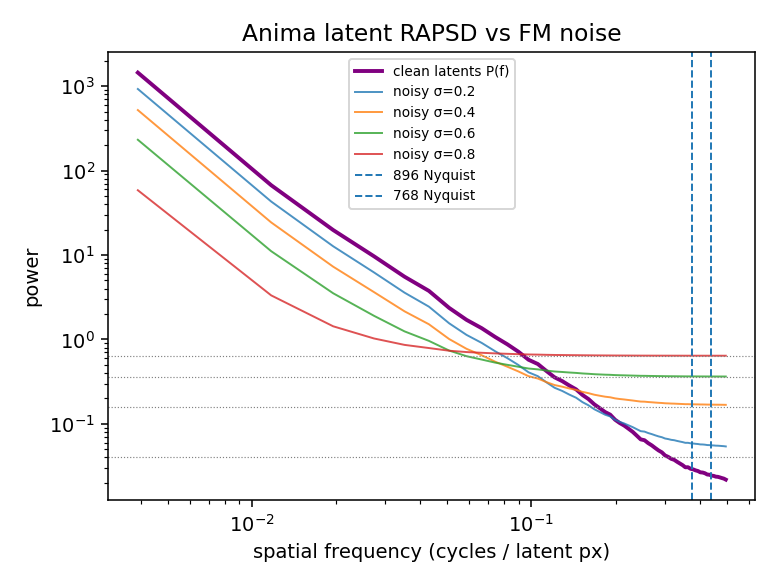
\includegraphics[width=\linewidth]{figs/rapsd_spectrum.png}
\caption{Latent RAPSD against the flow-matching noise floor at four
noise levels; dashed lines mark the demoted grids' Nyquist cuts.}
\label{fig:rapsd}
\end{subfigure}\hfill
\begin{subfigure}[t]{0.49\textwidth}
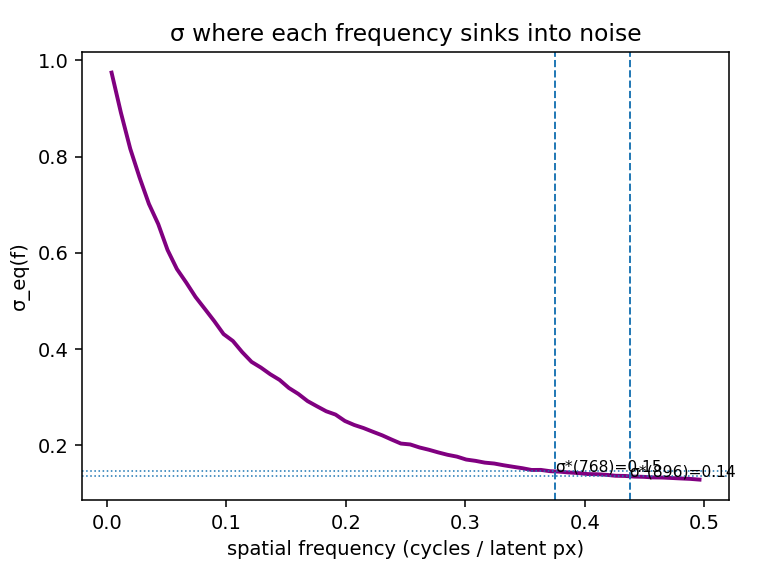
\includegraphics[width=\linewidth]{figs/rapsd_crossover.png}
\caption{The equal-power slice $\sigma_{\mathrm{eq}}(f)$ of the spectral
family. Predicted $\sigmastar$: $0.136$ / $0.146$ / ${\sim}0.20$ for
demotion to 896 / 768 / 512.}
\label{fig:sigmaeq}
\end{subfigure}
\caption{The spectral account, computed from the measured RAPSD and
transported to the training question (\S\ref{sec:null}): safety would
be predicted from $\sigma \approx 0.14$. Against the measurement
(Fig.~\ref{fig:verdict}) no tolerance reproduces the pattern
(Table~\ref{tab:null}): the equal-power crossover is off by
${\sim}3.5\times$, and the $2\times$ downscale, predicted safe by every
tolerance, is measured unsafe at every noise level.}
\label{fig:spectrum}
\end{figure}

\paragraph{The spectrum.}
The Qwen-Image VAE's latents are high-frequency-quiet ($P(f) < 1$ above
$f \approx 0.16$ cycles/latent-pixel; latent variance $0.42$), giving the
equal-power crossovers $\sigmastar(896) = 0.136$,
$\sigmastar(768) = 0.146$, $\sigmastar(512) \approx 0.20$, with tight
per-image spread (p10--p90 ${\approx}\,0.11$--$0.16$): the spectral
crossover is image-generic, and at that tolerance demotion would be safe
over almost the entire $\sigma$ axis (Fig.~\ref{fig:spectrum}).

\paragraph{The tolerance family, scored at the boundary level.}
Table~\ref{tab:null} instantiates Eq.~\ref{eq:spd} on the measured
latent spectrum ($P$ at the $896/768/512$ cuts $=$
$0.025/0.029/0.065$). Because the latents are high-frequency-quiet, $P$
barely varies across the cuts and the family is compressed: the spread
between the mildest and harshest route remains below ${\sim}0.13$ in
$\sigma$ at every tolerance. No row reproduces the measured pattern of
\S\ref{sec:instrument}: the $\delta$ that matches the measured $896$
boundary ($\delta = 0.025$) predicts $768$ safe at $0.52$ and $512$
safe at $0.62$, while SPD's own published $\delta = 0.01$ predicts all
three routes safe by $0.72$, and no $\delta$ anywhere in the family
can produce a $\sigma$-independent floor.

\paragraph{Which tolerance?}
Eq.~\ref{eq:spd} needs a $\delta$, and it is worth asking where one could
legitimately come from. SPD's published $\delta = 0.01$ is an
inference-side choice, selected on a speed--quality Pareto ablation over
generated images \citep{xiao2026spd}; nothing ties it to gradients.
Machine precision is not the relevant floor either: bf16 rounding on
unit-scale per-band amplitudes injects power of order $10^{-5}$ or below,
orders of magnitude beneath any boundary-moving tolerance. Our setting,
however, fixes a tolerance \emph{by construction}: the demotion recipe
pays a resize--VAE-encode round trip whose latent error has measurable
per-band power $D(f)$ (the same pipeline noise the re-encoding control
prices at the gradient level), and $D$ is expressed in exactly
Eq.~\ref{eq:spd}'s units (per-band power against unit noise). Band
content below $D(f_{\mathrm{cut}})$ is invisible to the substitution
pipeline even with no resolution change, so
$\delta_{\reenc}(e) := D(f_{\mathrm{cut}}(e))$ anchors the family with zero
free parameters. Measured on the probe set ($N{=}40$, same
resize--encode chain as the re-encoding control), the anchor is tiny
and image-generic: $\delta_{\reenc} \approx 1.0\times10^{-5}$ at all
three cuts (p10--p90 within $[1, 2]\times10^{-5}$; per-band SNR
$P(f_{\mathrm{cut}})/D(f_{\mathrm{cut}}) \approx 2.5$--$4.4\times10^{3}$),
pushing the anchored boundaries to $t^{*} \approx 0.98$ on every route
(Table~\ref{tab:null}). The parameter-free anchor is therefore maximally
conservative and still structurally wrong in both directions at once:
it moves all three boundaries together (spread $< 0.01$), it certifies
the measured-safe route only above $\sigma \approx 0.98$ where the
measurement certifies it from $\sigma \approx 0.5$, and, like every
member of the family, it predicts that the $2\times$ downscale becomes
safe, when no noise level does. Either way the confrontation does not
hinge on the choice: the structural failures --- ratio-only
boundaries, and a finite safe boundary for every route --- are
$\delta$-independent.

\begin{table}[t]
\caption{The spectral account (Eq.~\ref{eq:spd}) instantiated on the
measured latent spectrum: predicted safe boundaries $t^{*}$ per route as
the tolerance $\delta$ sweeps its range. SPD's published default is
$\delta = 0.01$; the
equal-power slice is the classical crossover; $\delta_{\reenc}$ is the
measured re-encode noise floor, the zero-free-parameter anchor fixed by
our own pipeline. No row reproduces the
measured pattern (last line; \S\ref{sec:map}): the $\delta$ that matches
the safe route's
boundary predicts both failing routes safe by $\sigma = 0.63$, and no
$\delta$ can produce a floor.}
\label{tab:null}
\centering
\small
\setlength{\tabcolsep}{4pt}
\begin{tabular}{lcccl}
\toprule
tolerance $\delta$ & $1024{\to}896$ & $1024{\to}768$ & $1024{\to}512$ & \\
\midrule
$(1+P_\omega)/2$ (equal power) & $0.14$ & $0.15$ & $0.20$ & classical crossover \\
$0.05$ & $0.41$ & $0.43$ & $0.53$ & \\
$0.025$ & $0.50$ & $0.52$ & $0.62$ & tuned to the measured $896$ gate \\
$0.01$ & $0.61$ & $0.63$ & $0.72$ & SPD's published default \\
$0.005$ & $0.69$ & $0.71$ & $0.79$ & \\
$\delta_{\reenc} \approx 10^{-5}$ & $0.98$ & $0.98$ & $0.99$ & the parameter-free anchor \\
\midrule
\textbf{measured, debiased} & ${\approx}\,0.5$ &
none certified & unsafe, all $\sigma$ & floors $.02$--$.04$ / $.06$--$.09$ / ${\approx}\,.3$ \\
\bottomrule
\end{tabular}
\end{table}

\subsection{The floor is graph: three probes, one number}
\label{sec:floor}

\begin{table}[t]
\caption{The floor, debiased. \textbf{Endpoint}: at $\sigma{=}1$ the
input is exactly $\epsilon$ on every grid, so the input-mediated data
term vanishes by construction. \textbf{x-zero}: the image is removed
from input \emph{and} target; any surviving gap is pure graph-shape
sensitivity. Debiased draw-limit values $\dgap_\infty$ [bootstrap 95\%
CI over images] from nested draw sweeps (endpoint: $N{=}12$,
$D = 4 \ldots 64$; x-zero: $N{=}40$, $D = 4 \ldots 32$). The endpoint
and x-zero columns agree within CI at every route, and the account's
pre-registered kill switch (all endpoint gaps ${\approx}\,0$) does not
fire.}
\label{tab:floor}
\centering
\small
\begin{tabular}{lcc}
\toprule
route & endpoint $\dgap_\infty$ [95\% CI] &
x-zero $\dgap_\infty$ [95\% CI] \\
\midrule
native self-floor (cosine) & $1.005$ $[0.994, 1.016]$ & --- \\
re-encoding control & $-0.003$ $[-0.017, +0.008]$ & --- \\
$1024{\to}896$ & $+0.019$ $[+0.010, +0.030]$ & $+0.034$ $[+0.017, +0.058]$ \\
$1024{\to}768$ & $+0.056$ $[+0.043, +0.071]$ & $+0.074$ $[+0.053, +0.094]$ \\
$1024{\to}512$ & $+0.304$ $[+0.197, +0.424]$ & $+0.283$ $[+0.232, +0.332]$ \\
\bottomrule
\end{tabular}
\end{table}

Three designated probes
establish the graph term, and with it the premises of the
reduction. At the $\sigma = 1$ \emph{endpoint} the input is pure
$\epsilon$, identical in distribution across arms, so the
input-mediated data term is zero by construction; per
\S\ref{sec:branches}, the target-mediated share need \emph{not} vanish
there, so the endpoint alone does not isolate the graph term, and the
next two probes discharge that step empirically. The debiased endpoint
floors are $+0.019 / +0.056 / +0.304$ for $896/768/512$
(Table~\ref{tab:floor}); the $512$ value clears the pre-registered
confirmation bar ($\dgap_\infty \ge 0.15$) on $12$ of $12$ probe images
individually, so the token-count floor is not an estimator artifact.

The \emph{x-zero} probe removes the image from input \emph{and} target
everywhere, isolating pure graph-shape sensitivity, and its debiased
draw-limit gaps are statistically equal to the endpoint gaps at
\emph{every} route (Table~\ref{tab:floor}). The
\emph{target-strength sweep} closes the remaining loophole from the
$\alpha$ side: re-running the endpoint with target $\epsilon - \alpha x$,
$\alpha \in \{0, 0.25, 0.5, 0.75, 1\}$ ($N{=}12$, $D{=}16$, one run,
shared draws across $\alpha$), the paired debiased excess is
$\alpha$-flat at the well-conditioned anchors ($768$:
$+0.070 \pm 0.015$ at $\alpha{=}0$ versus $+0.049 \pm 0.010$ at
$\alpha{=}1$; $512$: $+0.269 \pm 0.041$ versus $+0.337 \pm 0.067$;
re-encoding control slope $+0.003$): no resolvable target-content
share \emph{in the angular estimand}. The interior points $\alpha \in [0.5, 0.75]$ are unreadable by
construction and excluded: there the native residual
$\alpha x - \hat{x}$ passes near cancellation, the gradient norm dips
($60 \to 33$) and the redraw floor falls to $0.87$, so the estimator
reads through a small gradient norm, the low-norm amplification of
\S\ref{sec:anatomy} surfacing along the $\alpha$ axis. Endpoint $\equiv$
x-zero $\equiv$ $\alpha$-flat: three independent probes converge on one
number per route.

\paragraph{Why the target term is angularly invisible: it lands
parallel.}
The $\alpha$-flatness is not a cancellation mystery, and it does not
mean the target-mediated share of \S\ref{sec:branches} is absent.
Because the objective is quadratic, $\bar g$ is \emph{affine} in
$\alpha$, so the exact target-mediated gradient
$t = \bar g(1) - \bar g(0)$ is computable from the endpoint arms with
zero draw noise beyond theirs; measuring it directly ($N{=}40$
endpoint, two independent draw sets) shows the term is real and large
--- $\|t_{\src}\| / \|\bar g_{\src}\| \approx 2.2$, so $J^{\!\top}$
does \emph{not} annihilate target content --- but demotion's change to
it, $\delta t = t_{\dem} - t_{\src}$, lands almost entirely
\emph{along} $\hat g_{\src}$: $\kappa_\parallel = -0.75 / -1.18 /
-1.86$ on $896/768/512$ against $\kappa_\perp = 0.09 / 0.14 / 0.20$,
an $8$--$9\times$ parallel dominance, reproducible across the
independent draw sets ($\delta t$ direction agreement $\ge 0.995$)
while the re-encoding control sits at the noise floor with an
irreproducible $\delta t$ direction. Demotion \emph{shortens} the
target-mediated gradient along $\hat g_{\src}$, severity-ordered
($\|t\| / \|\bar g_{\src}\|$: $2.2 \to 1.5 \to 1.1 \to 0.5$);
direction rotation appears only on the harshest route
($\cos(t_{512}, t_{\src}) = 0.74$ against $0.99/0.98$ for $896/768$).
The cosine gap is blind to a parallel rescaling (Eq.~\ref{eq:exact}),
and the orthogonal part enters only at second order,
$\kappa_\perp^2 / 2 \approx 0.004$--$0.02$, below the floors it would
have to move: the $\alpha$-flat scalar result stands \emph{because}
the target term lands parallel, not because it vanishes. (Per image
the orthogonal loading is ${\sim}10\times$ the aggregate's;
image-specific directions cancel in the mean, the same motif as the
residual-direction read of \S\ref{sec:anatomy}.) The endpoint gap
\emph{is} the graph floor as the angular estimand reads it, an
empirical result established at our operating point, not assumed by
construction.

How does the floor relate to the interior high-$\sigma$ bins? For $512$
the debiased window means ($+0.08$--$0.60$) sit at or above the floor,
as additivity requires. For $896$ and $768$ the floors ($0.02$--$0.04$
and $0.06$--$0.09$) are \emph{at or below} the interior bins'
certification resolution ($\epsstar = 0.03$--$0.08$ at $N{=}40$,
$D{=}8$): the endpoint sweeps resolve them only because their effective
draw budget is an order of magnitude larger. The claim ``the
high-$\sigma$ plateau is the floor'' therefore sharpens to: the floor is
what the plateau converges to when the data term dies and the estimator
is given enough draws to see it.

Two further exonerations. The re-encoding control sits at zero within CI
(debiased $-0.003$ $[-0.017, +0.008]$), so the VAE round trip is
not the cause; conversely, the round trip has
\emph{measurable} input-level error while its gradient cost is below
instrument resolution, so input-level error neither implies nor excuses
gradient-level cost. And a forward-only probe of the model's
caption-conditioned \emph{prior} across grids shows route distances that
are flat where the floors are strongly ordered, so the floor's
route-ordering lives in the Jacobian factor $J$, not in the model's
resolution-conditioned prior, and not in a training-distribution
discontinuity (the 1280 grid, absent from training, is no more distant
from 1024 than heavily trained adjacent pairs are from each other).

\subsection{The data branch: a route-uniform numerator over a U-shaped
denominator}
\label{sec:anatomy}

\paragraph{$m(\sigma)$ is route-uniform in amplitude: the
residual-level spectral prediction fails.}
Measuring the mean prediction residual
$\bar r = \mathbb{E}_\epsilon[\hat v - (\epsilon - x)]$ per grid and
$\sigma$ (the exact $r$ in $g = J^{\!\top} r$) shows a strong,
monotone $\sigma$-shape (cross-grid excess $0.89 \to 0.36$ in relative
$L_2$ from $\sigma{=}0.125$ to $1$) that is the \emph{same for every
route} within $\pm 0.02$, across routes whose gradient floors span $0$ to
$0.3$ and whose crossovers span $0.5$ to nonexistent (Appendix
Table~\ref{tab:residual}). This kills the residual-level prediction of
\S\ref{sec:null}: with no cross-frequency coupling, its mismatch is confined to
the destroyed band and ordered by destroyed-band energy, which differs
substantially across these routes; route-uniformity says the real
mismatch is carried by cross-band structure the diagonal model cannot
express. All route identity therefore lives in $J$, not in the prediction
error, a pre-registered contrast that would equally have falsified the
account's factorization had the residual curves been route-ordered;
instead it \emph{establishes} the shape factorization directly. The
decay is smooth, Wiener-like posterior shrinkage with no hard gate at
the spectral crossover: gap curves read as ``collapsed'' where the
data term sinks below the instrument's certification resolution, not
at $\sigma_{\mathrm{eq}}$.

A direction-resolved follow-up sharpens what ``route-uniform'' means:
the uniformity is a property of the \emph{amplitude} only. Saving the
per-image mismatch vectors and comparing $\Delta \bar r$ directions
with a split-half attenuation correction, non-adjacent route pairs are
near-orthogonal at low $\sigma$ (corrected cosine $0.00$--$0.08$ at
$\sigma \le 0.375$) with only a weak shared component at high $\sigma$
($+0.2$--$0.3$ at $\sigma \ge 0.875$); the top mode of a stacked SVD
carries $0.33$--$0.36$ of the energy against the $0.25$
rank-4-uniform baseline (a rank-one common mode would give
${\approx}\,1$); and cross-image direction consistency is zero at
every (route, $\sigma$) cell (max $+0.019$ at split-half
reliabilities $0.73$--$0.99$), so the mismatch direction is fully
image-specific --- refuting a grid-conditional composition prior
(``small canvas $\Rightarrow$ portrait framing'') as the carrier, at
least under full captions. What \emph{is} shared is scale and
spectral drift: $\Delta \bar r$ energy migrates toward low
frequencies as $\sigma$ rises (low-third share $0.40 \to 0.67$ by
$\sigma = 0.875$), composition-scale but per-image. The factorization
of Eq.~\ref{eq:twoterm} only ever consumes the norm
$m(\sigma) = \|\Delta \bar r(\sigma)\|$, so the account is untouched;
what sharpens is the open question, now ``why is only the
\emph{amplitude} universal when the directions are image- and
route-specific.'' A closed-form candidate for cross-band coupling per
se exists --- the flow posterior covariance, whose off-diagonal
$D_z v^*$ entries are
$-\big((1{-}\sigma)/\sigma^3\big)\,\mathrm{Cov}(x_\omega, x_{\omega'}
\mid z)$ \citep{xing2026divunc}, set to zero by the diagonal-Gaussian
premise ---
but its rank-one common-mode version is excluded by the SVD read
above.

\paragraph{$\|\bar g_{\src}(\sigma)\|$ shapes the curve.}
Because the gap is a cosine it measures a mismatch \emph{fraction}; the
total gradient norm is U-shaped in $\sigma$ ($2.6 \to 0.4$ at
$\sigma\!\approx\!0.3 \to 9.3$; Fig.~\ref{fig:estimator}): large at
high $\sigma$ where the model is pulling composition out of the prior
and the residual is image-scale, small in the mid-$\sigma$ refinement
regime, and inflated again at low $\sigma$ by irreducible $\epsilon$. A
monotone absolute mismatch divided by a U-shaped norm yields exactly the
measured interior-peaked gap curves: bin-mean gap tracks
$1/\|\bar g_{\src}\|$
(Spearman $+0.55$ to $+0.90$ across arms and runs, and within images),
and renormalizing by $\|\bar g_{\src}\|$ flips the anomalous
low-$\sigma$ dip into the monotone maximum in every arm of both runs,
the predicted $m/\|\bar g_{\src}\|$ shape. This is a post-hoc consistency analysis (so labeled): it
explains the \emph{shape}; all safety criteria stay in
cosine units, since direction is what a normalized optimizer consumes.

\paragraph{The governors: ratio sets the amplitude, absolute size sets
the floor.}
With the floor isolated, what orders the routes? Two probes give a clean
division of labor.
\emph{Absolute size, not ratio, sets the floor}: the route
$1280{\to}1024$ is \emph{more} aggressive by ratio ($0.80$) than
$896{\to}768$ ($0.857$, no certifiable window), yet its floor is
${\approx}\,0$ and it enters the re-encoding band at
$\sigma \gtrsim 0.75$, refuting any pure ratio rule for the floor,
and with it the spectral account's only degree of freedom. (The $896{\to}768$ read
is direct: re-run one tier down, the route fails its pre-registered bar
with a high-$\sigma$ residual ${\sim}2\times$ the $1024{\to}896$
plateau, at ratio $0.857$ against the passing $0.875$, while the
spectral family puts these two boundaries within $0.01$ of each other at every
tolerance; Appendix Table~\ref{tab:phase1a}.) Conversely the floor
grows monotonically as the \emph{target} grid shrinks
($0.02$--$0.04$ / $0.06$--$0.09$ / ${\approx}\,0.30$ at
target ${\sim}3{,}000 / 2{,}160 / 1{,}000$ tokens), consistent with
``floor $=$ how well the coarse graph approximates the fine graph's
computation.''
\emph{Ratio, not absolute size, sets the amplitude}: a synthetic
iso-severity route $1280{\to}1120$ (edge ratio $0.875$ exactly
matched to $1024{\to}896$, but $1.6\times$ its absolute target size)
reproduces the $1024{\to}896$ curve bin-for-bin and its crossover
$\sigmastar\!\approx\!0.5$, while the same-native $1280{\to}1024$ (ratio
$0.80$) separates and floors later (Appendix
Table~\ref{tab:isoseverity}). Amplitude follows ratio; with
$\Floor_{1120} \approx 0$ this completes the division: \emph{ratio sets
$A_e$; absolute target capacity sets $\Floor_e$}. The pre-registered
contrast (ratio-governed $\Rightarrow$ $\sigmastar \approx 0.5$;
capacity-governed $\Rightarrow$ earlier floor) discriminated cleanly.
Note what survives of the spectral account here: ratio \emph{is} the
right governor for the data term; its error is not its
governor but its scope, mistaking one term for the whole gap.

\subsection{Decomposing the floor: depth, and a positional share}
\label{sec:decomposition}

\paragraph{Depth, not module type.}
Splitting the probe gradients per module type ($15$ groups, including
separate rows of the fused QKV projections) and per block ($28$) shows the
floor concentrated in \emph{depth}: early blocks (0--9, peaking at 3--8)
carry ${\sim}3\times$ the late-block gap, uniformly across every module
type within a block (at $512/\sigma{=}1$, every type sits in
$0.22$--$0.31$; Appendix Table~\ref{tab:depth}). The mechanism
picture: the first ${\sim}10$ blocks build grid-calibrated token
statistics; the divergence propagates into every parameter type's gradient
in those blocks roughly equally, and deeper blocks inherit a washed-out
version. Notably, query and key projections show \emph{zero} excess over
value projections, which we initially read as refuting a
rotary-embedding mechanism. That inference was wrong, in an instructive
way.

\paragraph{$\Floor_e = \mathrm{RoPE}_e + \mathrm{Resid}_e$.}
Landing-side uniformity cannot localize \emph{origin}: a perturbation
originating in the position embedding propagates through the block and
lands on all module types. The discriminating experiment is the
origin-side intervention of \S\ref{sec:branches}: evaluate the demoted
grid with positionally-interpolated fractional rotary coordinates (patch
$i$ at $i \cdot H_{\src}/H_{\dem}$ per axis), making its
relative phase geometry exactly match native. At the $\sigma{=}1$
endpoint this \emph{erases} the $768$ floor (paired
$\Delta = +0.081$, $78\%$ of images improved) and removes ${\sim}30\%$
of the $512$ floor (paired $\Delta = +0.096$), while leaving the in-band
$896$ control untouched (Appendix Table~\ref{tab:pi}; the paired
$\Delta$s are same-grid contrasts at matched draws, in which the
finite-draw bias cancels to first order). Re-anchored against the
debiased floors: the $+0.081$ erasure accounts for essentially all of
the $768$ floor ($\mathrm{Resid}_{768} \approx 0$); against the $512$
floor of ${\approx}\,0.30$, the $+0.096$ erasure leaves a
$\mathrm{Resid}_{512} \approx 0.2$ bulk. The mild-route floor is mostly
a \emph{coordinate-system artifact}; the harsh-route bulk is a genuine
non-positional graph residue (attention-over-$N$ statistics,
sequence-length-dependent normalization, capacity). The capacity
governor of \S\ref{sec:anatomy} attaches to $\mathrm{Resid}_e$, as the
band-counting sketch anticipated. The attention-over-$N$ piece has
inference-side prior art: attention-entropy corrections derive
length-dependent temperatures to preserve the $\log N$ entropy term
\citep{li2025infoscale}, and TIDE applies the same dilution correction
jointly to resolution and diffusion timestep \citep{liu2026tide} ---
the closest prior work to a $\sigma$-gated resolution correction,
though on the inference side; our gate is training-side and set by
measured gradient safety, not by an entropy invariance. The $896$ route's small floor
($0.02$--$0.04$) sits below the PI probe's paired resolution and remains
undecomposed.

\paragraph{The floor as a ledger.}
Combining the designated probes, the floor decomposes additively, each
share measured by its own intervention:
\begin{equation*}
\Floor_e \;=\;
\underbrace{\reenc}_{{\approx}\,0 \text{ by control}}
\;+\; \underbrace{\text{target content}}_{\text{lands }\parallel\;
\hat g_{\src}\text{: angular share}\,{\approx}\,0}
\;+\; \underbrace{\mathrm{RoPE}_e}_{\text{erased by PI at }\sigma{=}1}
\;+\; \underbrace{\mathrm{Resid}_e}_{\text{remainder}}
\end{equation*}
with totals $0.02$--$0.04$ ($896$; undecomposed),
${\approx}\,0.07$ ($768$; $\mathrm{RoPE}$ the large majority,
$\mathrm{Resid} \approx 0$), and ${\approx}\,0.30$ ($512$;
$\mathrm{RoPE} \approx 0.10$, $\mathrm{Resid} \approx 0.20$). One
caveat on the first share: the re-encoding control
(native decode$\to$re-encode) is a \emph{proxy} for the pipeline cost
demotion actually pays (source downscale$\to$encode); the
demote--re-promote arm (\S\ref{sec:confronted}) closes that gap
empirically. The data leg's orthogonal magnitude $|B^{\perp}|$
measured against the re-encoded reference agrees with the
native-referenced read to ${\sim}4\%$ at the signal-carrying
low-$\sigma$ bins (worst $\pm 23\%$ only in bins where $B$ is already
small), so the shared downscale$\to$encode pipeline cost is a minor
share of the data intervention (Appendix Table~\ref{tab:e9ledger}).

\paragraph{The positional share is a noise-regime artifact only.}
A $\sigma$-resolved follow-up closes the tempting route this opens
(training $1024{\to}768$ through interpolated coordinates): with image
content in the input, the stretched forward is \emph{off-manifold}; the
interpolated arm is \emph{worse} than the plain demoted arm through
$\sigma \in [0.56, 0.81]$ (paired $-0.05$ to $-0.11$) and wins only at
$\sigma \ge 0.94$. The floor's positional share is erasable only where
the input is noise-dominated, so the decomposition is a mechanism finding,
not a training lever; the data term of the $768$ route is in any case
fatal on its own ($+0.09$--$0.22$ over control across the window). A
frequency-\emph{selective} banded alignment does survive in-window
(\S\ref{sec:trainer}).

\subsection{The account confronted: held-out routes and the reduction's
domain}
\label{sec:confronted}

The probes so far test the account's \emph{structure}. The remaining
test is whether it is a \emph{predictive} theory: fit the reduced
account on three routes, then predict two held-out routes from
the governors alone (Fig.~\ref{fig:e5}). Fit routes: $\{1024{\to}896,\ 1024{\to}512,\ 1280{\to}1120\}$;
held-out: $\{1024{\to}768,\ 1280{\to}1024\}$. Per fit route the excess
curve $\bgap_e(\sigma)$ is fit with a route amplitude and floor on
the measured route-uniform amplitude $m(\sigma)$ and each run's own
$\|\bar g_{\src}(\sigma)\|$;
two governor models ($A(\mathrm{ratio})$ interpolating the fitted
amplitudes, and an exponential floor law $F(n) = F_0\,e^{-n/\tau}$ in
target tokens $n$) then generate the held-out predictions with zero
per-route freedom. Pass criteria were pre-registered in the analysis
script before the numbers.

\paragraph{Held-out results.}
All four pre-registered gates fire:
(i)~held-out $1024{\to}768$: RMSE $0.093$, \emph{better than an
oracle quadratic fit on the held-out data itself} ($0.105$), and better
than the spectral account on its committed region
($\sigma > \sigma_{\mathrm{eq}}$,
where it predicts gap $0$: RMSE $0.164$ vs $0.096$ ours);
(ii)~held-out $1280{\to}1024$: RMSE $0.092$ vs oracle $0.056$, inside
the pre-registered $2\times$ gate;
(iii)~the ratio governor holds at the amplitude level: the two
ratio-$0.875$ routes agree at $z = 0.14$ despite a $1.6\times$
difference in target capacity;
(iv)~the floor law $F(n) = 0.70\,e^{-n/1041\,\mathrm{tok}}$, fit on the
$512$ and $896$ floors, predicts $F(4825) = +0.007$ for the $1120$ grid
(fitted $+0.002$) and $F(2160) = +0.088$ for the held-out $768$ grid,
against a measured endpoint floor of $+0.092 \pm 0.012$. The point
estimate lands exactly, but its own sampling spread is wide: a
full-pipeline bootstrap (Fig.~\ref{fig:e5}; \S\ref{sec:trainer}) puts
$F(2160)$ at $68\%$ $[+0.042, +0.091]$, consistent at the interval's
upper edge, so the licensed read is agreement, not exactness. A
post-hoc leave-$896$-out addendum (so labeled) re-derives the governors
from $512$+$1120$ alone and predicts the $896$ floor at $+0.019$ against
the measured $+0.019$ $[+0.010, +0.030]$: the floor law is correct on
both floors outside its fit set.

\paragraph{The floor law is a calibrated interpolation, not a
mechanism.}
Two anchors and one held-out check cannot identify a functional form,
and the cosine gap is the wrong scale to fit one in: it saturates
(Eq.~\ref{eq:exact}). Refitting the same anchors in the unsaturated
perturbation-energy units,
$\kappa_{\mathrm{eff}}^2 = (1-F)^{-2} - 1$, gives
$\tau \approx 860$ tokens and predicts $F(2160) = +0.096$, equally
consistent with the measured $+0.092 \pm 0.012$; and the same two
anchors pushed through $e^{-\sqrt{n}/\ell}$ or a power law $n^{-p}$
predict $+0.085$ and $+0.075$ --- every form lands within the union of
the measured CI and the prediction's own bootstrap spread
(\S\ref{sec:trainer}). The exponential is therefore one member of a
candidate family $\{e^{-n/\tau},\ e^{-\sqrt{n}/\ell},\ n^{-p}\}$ our
operating points cannot distinguish, and the mechanical reading of
$\tau$ ($\approx 860$--$1040$ tokens across the two unit
conventions) as an effective-rank decay length of the early-block
gradient operator is a hypothesis, not a law. It is a discriminable
one: a spectral-tail account predicts a source-capacity dependence
$F \propto e^{-n/\tau} - e^{-n_0/\tau}$ where the
absolute-target-capacity governor of \S\ref{sec:anatomy} predicts
none (at our operating points the secant correction sits within
calibration slack, so the existing anchors do not discriminate); the
designated run is a fixed-target, varied-source token ladder, not yet
scheduled.

\paragraph{Functional form: the exact link headlines.}
Refitting the same pipeline under three forms for the data term (a
fitted power $A\,m/G^p$ with $p$ shared and free, the derived quadratic
$A\,(m/G)^2$, and the exact angular link, Eq.~\ref{eq:exact})
resolves the form question in the geometry's favor twice over
(Appendix Fig.~\ref{fig:e51280}; on the fit routes the three forms are
visually indistinguishable, so Fig.~\ref{fig:e5} carries the headline
form only). First, the free exponent's own optimum lands on
$p = 2.00$ exactly: the ``empirical'' power form recovers the derived
quadratic on its own. Second, the exact link is the best held-out
predictor (mean RMSE $0.071$ vs $0.093$--$0.094$ for the other two),
and its entire margin comes from the $1280{\to}1024$ route (RMSE
$0.049$ vs ${\approx}\,0.095$; Appendix Fig.~\ref{fig:e51280}): the
quadratic systematically
\emph{overshoots} that route's mid-$\sigma$ peak, and the exact link's
saturation removes the overshoot; what a first analysis had booked as
convexity in the $A(\mathrm{ratio})$ governor was quadratic-form error.
The governors are form-invariant (floor law $F(2160) = +0.087$--$0.088$
under all three; ratio-twin $z \le 0.44$). Per the ledger of
\S\ref{sec:geometry}: Eq.~\ref{eq:exact} is the best empirical
predictor (empirical through its linear loading $c_e\,m$), and the
derived quadratic is its small-$\kappa$ limit: one geometry at two
orders, not two competing models.

\paragraph{Stated limits.}
The prediction is \emph{not} within certification resolution anywhere
($\chi^2$/bin $7.6$--$9.2$ held-out under the quadratic): the licensed
claim is shape, magnitude class, and governors at ${\sim}0.07$--$0.09$
RMSE, not ``predicts within $\epsstar$.'' And the
$A(\mathrm{ratio})$ interpolation rests on two distinct ratio values.

\paragraph{The reduction's domain: one signed failure, and its
signature.}
The $768$ route's mid-$\sigma$ window is the reduction's one structural
failure, and its shape is diagnostic. Measured excess sits at zero
across $\sigma \in [0.56, 0.94]$, \emph{below} the predicted
$\Floor_{768} \approx 0.09$ and outside the bootstrap $95\%$ band
(Fig.~\ref{fig:e5}). This is structural, not sampling noise: a positive
two-term form cannot produce a gap under its own floor, under any
coefficients. In the four-term
expansion (Eq.~\ref{eq:fourterm}) a gap below the floor admits exactly
two mechanisms, and we pre-registered both ahead of the direct probe:
either (i)~the projected interaction is negative in the window,
$I_{768}(\sigma) < 0$ --- in which case an amplitude-matching account
predicts the window center sits where the two perturbation legs have
equal orthogonal magnitude, a testable localization --- or (ii)~the
graph share is itself $\sigma$-dependent, $F_{768}(\sigma)$ collapsing
below its endpoint value in-window, which would rewrite assumption
(iii) rather than (ii). Either way a named assumption fails exactly
where the account says it can, and the derived four-term form
represents the failure rather than excusing it. The window therefore
\emph{delimits the reduction's domain}. One honesty note on the probe
design: the scalar read we originally planned,
$\gap_{\mathrm{demote}} - \gap_{\mathrm{repromote}} - \Floor_e$,
cannot arbitrate --- it estimates $I(\sigma) + [F(\sigma) - F(1)]$
plus higher-order terms, conflating the two branches. The designated
direct test is therefore vector-resolved: the demote--re-promote
probe stores arm-mean gradients and reads the data, graph, and
interaction shares per (route, $\sigma$-bin) from the interventional
split $B = \bar g_{\mathrm{repromote}} - \bar g_{\src}$,
$C = \bar g_{\mathrm{demote}} - \bar g_{\mathrm{repromote}}$
($S = \|B^{\perp}\|^2/2\|\bar g\|^2$,
$F = \|C^{\perp}\|^2/2\|\bar g\|^2$,
$I = \langle B^{\perp}, C^{\perp}\rangle/\|\bar g\|^2$, with
cross-draw-set inner products to cancel shared-noise bias and exact
counterfactual angles alongside the quadratic ledger; instrument
details and the full ledger in Appendix Table~\ref{tab:e9ledger}).

\paragraph{The probe, run: branch (i), negative interference.}
The data picks branch (i), with the pre-registered localization
confirmed. $I_{768}(\sigma) < 0$ at every bin ($-0.31$ at
$\sigma = 0.56$, shrinking in magnitude to $-0.014$ by
$\sigma = 0.94$), with the two legs' orthogonal components near
anti-parallel in-window
($\rho = \cos(B^{\perp}, C^{\perp}) \approx -0.93$; the sign is robust
to the cross-set debiasing --- same-set $-0.39$ vs cross-set $-0.31$
at the first bin). Branch (ii) did not fire: $F_{768}(\sigma)$
decreases monotonically to its endpoint value ($0.200 \to 0.004$) and
never drops below it in-window, so the $\sigma{=}1$ endpoint reads of
\S\ref{sec:floor} are untouched. The amplitude-matching localization
lands where branch (i) predicts it: $|B^{\perp}|/|C^{\perp}| = 0.98$
at the $\sigma = 0.688$ bin, putting the predicted window center at
$\sigma \approx 0.69$, interior to the measured $[0.56, 0.94]$ window.
The anti-parallel geometry itself is universal ---
$\rho \in [-1.24, -0.62]$ across every route and bin --- so what
distinguishes the routes is amplitude matching, not sign: $896$ is
matched but low-amplitude (net $S{+}F{+}I \le +0.012$), $768$ is
matched at mid-window ($\le +0.029$), and $512$ is
amplitude-mismatched at low $\sigma$
($|C^{\perp}|/|B^{\perp}| \approx 1.8$, net up to $+0.20$).

\paragraph{How much of the gap the interference erases.}
Because $\bar g_{\mathrm{dem}} = \bar g_{\src} + B + C$ by
construction, the realized demotion distance is exactly the
counterfactual angle $h(B{+}C)$, where
$h(X) = 1 - \cos(\bar g_{\src},\, \bar g_{\src} + X)$ is the distance
the perturbation $X$ alone would produce; $h(B)$, $h(C)$, and
$h(B{+}C)$ are all computable from the stored arm means, so each
account's predicted-to-realized ratio is direct. The no-interference
scalar account $S{+}F$ overpredicts the realized in-window gap
$2.4$--$3.8\times$ at $768$ ($1.6$--$5.8\times$ at $896$,
$1.2$--$3.0\times$ at $512$); the fully additive counterfactual
$h(B) + h(C)$ overpredicts $3.5$--$8\times$ --- the realized
$h(B{+}C)$ is only ${\sim}20$--$30\%$ of the additive sum in-window,
i.e.\ roughly three quarters of the additively-predicted gap is
erased by the interference. That is the quantitative content of
branch (i); the vector account $B{+}C$ is exact by construction ---
including $I$ is what removes the overprediction. One unit-honesty
caveat: in-window $|B^{\perp}|, |C^{\perp}| \approx
0.5$--$1.0\,\|\bar g_{\src}\|$, outside the quadratic truncation's
domain, and the truncated ledger $S{+}F{+}I$ correspondingly
\emph{under}predicts realized magnitudes ${\sim}3$--$4\times$ (median
ratio $0.24\times$). The ledger therefore licenses sign,
decomposition, and window localization; gap magnitudes are quoted
from the exact counterfactuals $h(\cdot)$ throughout.

\paragraph{The spectral account, scored.}
Against our account's discriminating predictions, the
spectral account loses each one it is party to: the boundary pattern is
$\{{\approx}\,0.5$, no certifiable window, certifiably unsafe
everywhere$\}$ (\S\ref{sec:phenomenon}); gaps persist at pure-noise
input, equal to the floor and to the image-free control
(\S\ref{sec:floor}); ratio governs the amplitude while absolute size
governs the floor (\S\ref{sec:anatomy}); the residual curves are
route-uniform in amplitude under route-ordered gaps
(\S\ref{sec:anatomy}); and the
curve shape follows the $m/\|\bar g_{\src}\|$ read, not per-band SNR. The account also
retrodicts the observations that motivated no probe:
(i)~$\sigmastar \approx 0.5$ rather than $0.14$: the crossover is
where the data term sinks below certification resolution, a property of
the ratio, so the $3.5\times$ discrepancy is expected, not anomalous;
(ii)~the $896{\to}768$ failure (the $768$-grid floor alone fills the
certifiable margin, so no $\sigma$-gate can rescue it);
(iii)~$1280{\to}1024$ flooring \emph{later} ($\sigmastar \approx 0.75$)
but cleanly (harsher ratio $\Rightarrow$ larger $A_e$; large target
$\Rightarrow$ $\Floor \approx 0$), the single observation that breaks
both pure-ratio and pure-capacity route-ordering stories.

\begin{figure}[t]
\centering
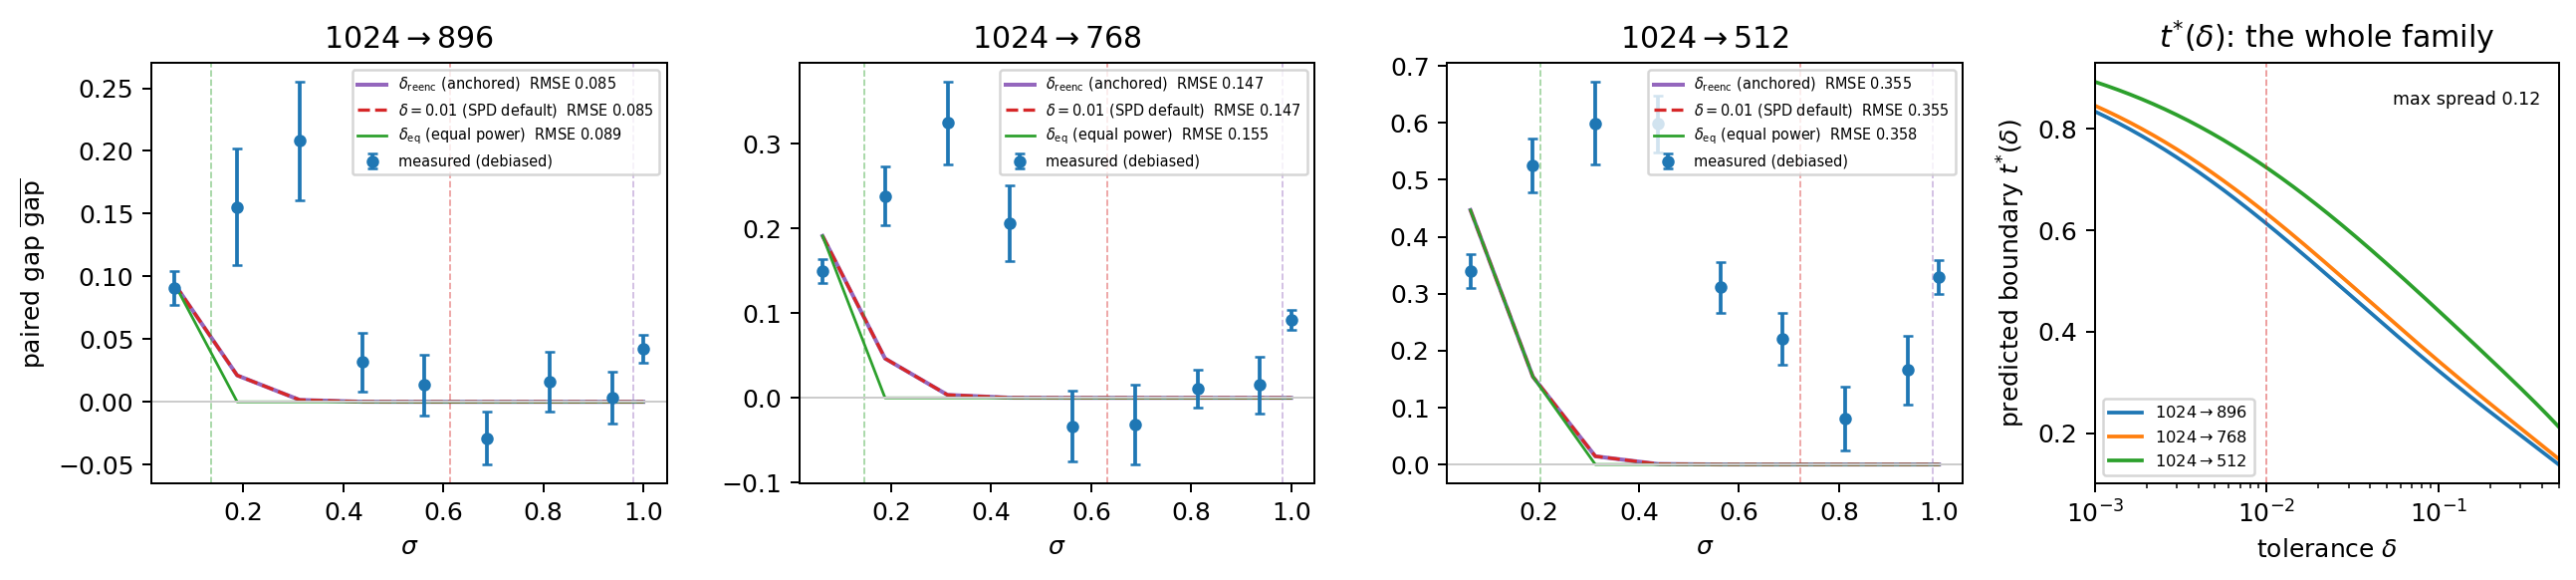
\includegraphics[width=\linewidth]{figs/e83_overlay.png}
\caption{The spectral account at the curve level. Left three panels:
measured debiased curves against the account transported through our
bridge --- the diagonal model's destroyed-band mean-residual mismatch
on the measured spectrum, through the measured
$\|\bar g_{\src}(\sigma)\|$ with a single gain calibrated on the one
safe route ($1024{\to}896$) and no floor (the family expresses none)
--- gated at $t^{*}(\delta)$ (dashed verticals) for the equal-power
slice, SPD's published default $\delta = 0.01$, and the measured
anchor $\delta_{\reenc}$. The transported curve dies by
$\sigma \approx 0.35$ on every route, so the default and anchored
gates act on an already-zero curve and their lines coincide.
Right: the boundary family $t^{*}(\delta)$ on the measured spectrum;
maximum route spread $0.125$ in $\sigma$ over
$\delta \in [10^{-3}, 0.5]$. Unit honesty: these curves are
\emph{the spectral account read through our bridge}, since it emits
residual units only.}
\label{fig:e83}
\end{figure}

The curve-level overlay (Fig.~\ref{fig:e83}) completes the
confrontation, and it fails in both directions at once, at every
tolerance. In-window, the transported family cannot produce the
measured mid-$\sigma$ structure: the latents are high-frequency-quiet,
so the model's destroyed-band mismatch is concentrated below
$\sigma \approx 0.3$ and the predicted curve is near zero exactly
where the measured curves peak (RMSE $0.147$ at $768$ and $0.355$ at
$512$, against $0.093$ held-out and $0.093$ in-sample for our
account) --- and because the curve has already died, every tolerance
from the equal-power slice to the measured anchor scores within
$0.01$ RMSE of every other: $\delta$, the family's one degree of
freedom, is inert at the curve level. Above each tolerance's
committed boundary, where every family member predicts exactly zero,
the floor persists: committed-region RMSE $0.027/0.049/0.218$ for
$896/768/512$ at SPD's default. Both reads are insensitive to the
residual-shape choice in the transport (per-draw vs mean-residual
within $10\%$; identical committed-region numbers), and the sweep
panel is the continuous form of Table~\ref{tab:null}'s rows
(analysis in \texttt{e83\_bridge.py}).

A corollary worth stating plainly: the safety of $1024{\to}896$ is an
\emph{empirical smoothness statement about this network's function across
nearby token counts}, not an information-theoretic statement about the
data. There was no a priori reason to expect a universal ratio
invariant.

